\section*{Aufgabe 5.1}
Im Folgenden wurde mittels der Fourier-Analyse eine Möglichkeit der Bildkomprimierung
getestet. Das verwendete Bild ohne Veränderungen ist in \fref{orig} abgebildet.

\begin{figure}[htb]
\centering
  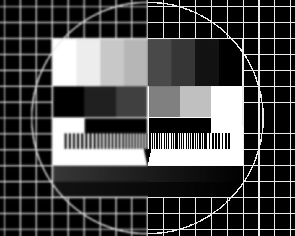
\includegraphics[width=0.7\textwidth,keepaspectratio]{../tmp/testbild.pdf}
  \caption{Orginales Bild ohne Komprimierung}
  \label{fig:orig}
\end{figure}

\section*{Aufgabe 5.1a)}

Zunächst wurde eine Funktion \lref{cut_rect} geschrieben, die den Rand des Graustufen-Bildes
schwärzt, die Pixel also auf 0 setzt. Die Breite wird hierbei in Abhängigkeit
des Kompressionsparameters $ρ \in ]0,1]$ so eingestellt, dass $hb\cdot ρ^2$
nicht-triviale Pixel verbleiben, wobei $h$ die Höhe und $b$ die Breite des
Bildes in Pixeln ist.

Wird die Funktion aus \lref{cut_rect} unter Verwendung von $ρ^2 = 0.4$ auf das
Bild in \fref{orig} angewendet, so erhält man die in \fref{1a} gezeigte Abbildung.
\lstinputlisting[firstline=1,lastline=8,firstnumber=1,label=lst:fft-test,caption={blatt5.m}]{../code/blatt5.m}
\lstinputlisting[firstline=1,lastline=10,firstnumber=1,label=lst:cut_rect,caption={cut\_rect.m}]{../code/cut_rect.m}

\begin{figure}[htb]
\centering
  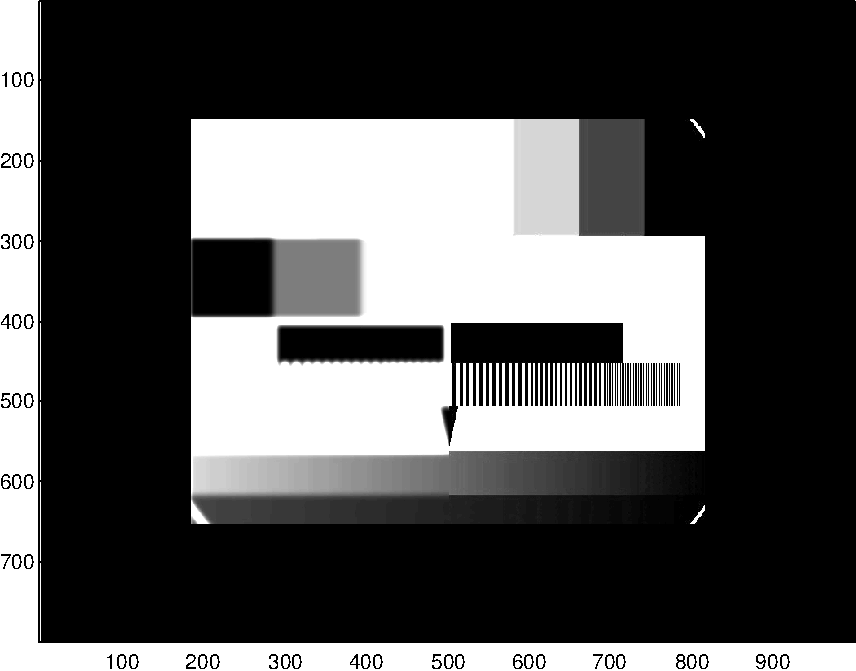
\includegraphics[width=0.7\textwidth,keepaspectratio]{../tmp/eins_a-crop.pdf}
  \caption{Bild mit Rand bei $ρ^2 = 0.4$}
  \label{fig:1a}
\end{figure}

Wie man erkennen kann, wurde abgesehen von der gewünschten Rahmen-Erzeugung
auch der innere Bereich des Bildes verändert, was allerdings nicht ein Effekt der
Beschneidung ist, sondern vermutlich auf die begrenzte Auflösung der Farbskala 
zurückzuführen ist. Daher sind beispielsweise die in der Bildmitte befindlichen
hellgrauen Blöcke im transformierten Bild nicht mehr zu finden. 

\section*{Aufgabe 5.1b)}
Für die folgenden Aufgaben wurden die in Matlab zur Verfügung stehenden 
Fast-Fourier-Transformationsfunktionen \texttt{fft, ifft, fft2, ifft2} benötigt.
Zunächst wurde getestet, wie diese funktionieren, indem mit einfachen Vektoren und
Matrizen eine Hin- und eine Rücktransformation durchgeführt wurde, wie in 
\lref{fft-test} gezeigt.
\lstinputlisting[firstline=10,lastline=23,firstnumber=10,label=lst:fft-test,caption={blatt5.m}]{../code/blatt5.m}

Der zugehörige Output ist in \lref{fft-test-output} gezeigt.
\begin{lstlisting}[caption=Output des Beispielaufrufs,label=lst:fft-test-output]
a =

    0.0759
    0.0540
    0.5308
    0.7792
    0.9340


a_fft =

   2.3738          
  -0.6786 + 0.9830i
  -0.3186 + 0.2811i
  -0.3186 - 0.2811i
  -0.6786 - 0.9830i


a_2 =

    0.0759
    0.0540
    0.5308
    0.7792
    0.9340


a_fftshift =

    0.7792
    0.9340
    0.0759
    0.0540
    0.5308


a_ifftshift =

    0.0759
    0.0540
    0.5308
    0.7792
    0.9340


A =

    0.1299    0.1622    0.6020    0.4505    0.8258
    0.5688    0.7943    0.2630    0.0838    0.5383
    0.4694    0.3112    0.6541    0.2290    0.9961
    0.0119    0.5285    0.6892    0.9133    0.0782
    0.3371    0.1656    0.7482    0.1524    0.4427


A_fft =

  11.1456            -0.8578 + 0.2117i  -0.9221 + 1.6125i  -0.9221 - 1.6125i  -0.8578 - 0.2117i
  -0.5132 - 0.6404i   0.6573 - 1.2749i  -0.1080 + 1.1941i  -0.2687 + 0.1951i   0.3350 - 1.9203i
   0.3664 + 0.1807i  -1.9259 + 1.5904i  -1.8499 + 0.0229i   1.4279 - 0.0361i  -0.2900 - 0.2633i
   0.3664 - 0.1807i  -0.2900 + 0.2633i   1.4279 + 0.0361i  -1.8499 - 0.0229i  -1.9259 - 1.5904i
  -0.5132 + 0.6404i   0.3350 + 1.9203i  -0.2687 - 0.1951i  -0.1080 - 1.1941i   0.6573 + 1.2749i


A_2 =

    0.1299    0.1622    0.6020    0.4505    0.8258
    0.5688    0.7943    0.2630    0.0838    0.5383
    0.4694    0.3112    0.6541    0.2290    0.9961
    0.0119    0.5285    0.6892    0.9133    0.0782
    0.3371    0.1656    0.7482    0.1524    0.4427


A_fftshift =

    0.9133    0.0782    0.0119    0.5285    0.6892
    0.1524    0.4427    0.3371    0.1656    0.7482
    0.4505    0.8258    0.1299    0.1622    0.6020
    0.0838    0.5383    0.5688    0.7943    0.2630
    0.2290    0.9961    0.4694    0.3112    0.6541


A_ifftshift =

    0.1299    0.1622    0.6020    0.4505    0.8258
    0.5688    0.7943    0.2630    0.0838    0.5383
    0.4694    0.3112    0.6541    0.2290    0.9961
    0.0119    0.5285    0.6892    0.9133    0.0782
    0.3371    0.1656    0.7482    0.1524    0.4427
\end{lstlisting}

Wie man erkennen kann, sind die Vektoren und Matrizen nach zwei Transformationen
gleich den hineingesteckten Objekten, sodass die grundlegende Funktionalität als
gegeben angenommen werden kann.

Weiterhin wurden die Funktionen \texttt{fftshift} und \texttt{ifftshift}
untersucht (siehe \lref{fft-test}). Diese führen zunächst eine Hin- bzw. Rücktransformation
durch und verschieben die $k$-Werte in der Art, dass pro Zeile und Spalte die 
zu $k=0$ gehörenden Werte in die Mitte gelangen. Dies entspricht einer Symmetrisierung.
Die Funktion \texttt{ifftshift} macht diese Symmetrisierung wieder rückgängig, um
die ursprüngliche Matrix wiederzubekommen.

Die beiden Funktionen \textcolor{red}{unterscheiden} sich aufgrund der Nichtlinearität der Abhängigkeit
von $x$ und $k$. (oder: octave- help fftshift -> laenge spielt eine rolle)


\section*{Aufgabe 5.1c)}
In dieser Teilaufgabe wurde das Bild mit der in \lref{cut_rect} gezeigten Funktion für
ϱ²-Werte von $0.1$ (\fref{pic_trafo_0_1}) und $0.5$ (\fref{pic_trafo_0_5})
transformiert und im $k$-Raum beschnitten.

\begin{figure}[htb]
\centering
  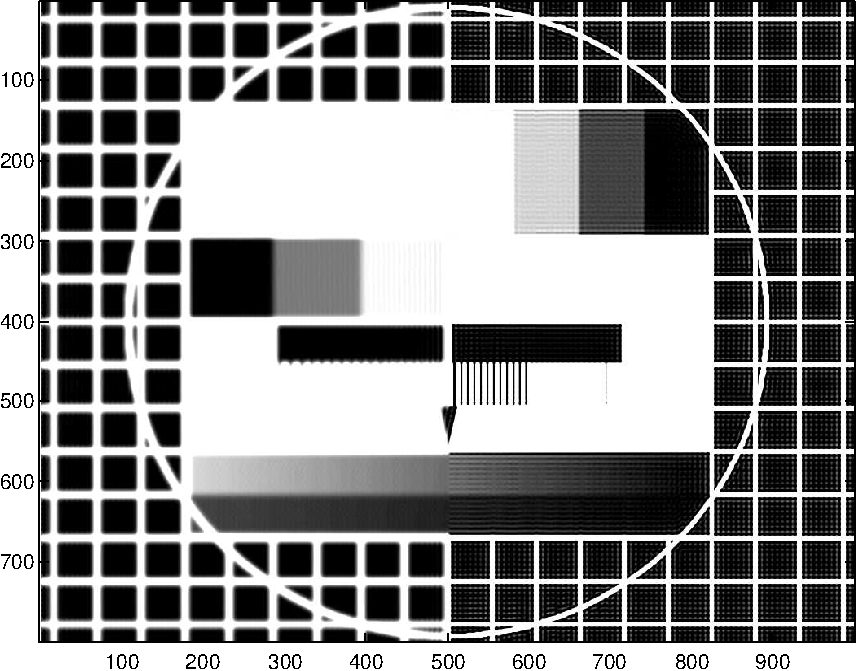
\includegraphics[width=0.7\textwidth,keepaspectratio]{../tmp/eins_c_0_1-crop.pdf}
  \caption{Bild mit Rand bei $ρ^2 = 0.1$}
  \label{fig:pic_trafo_0_1}
\end{figure}

\begin{figure}[htb]
\centering
  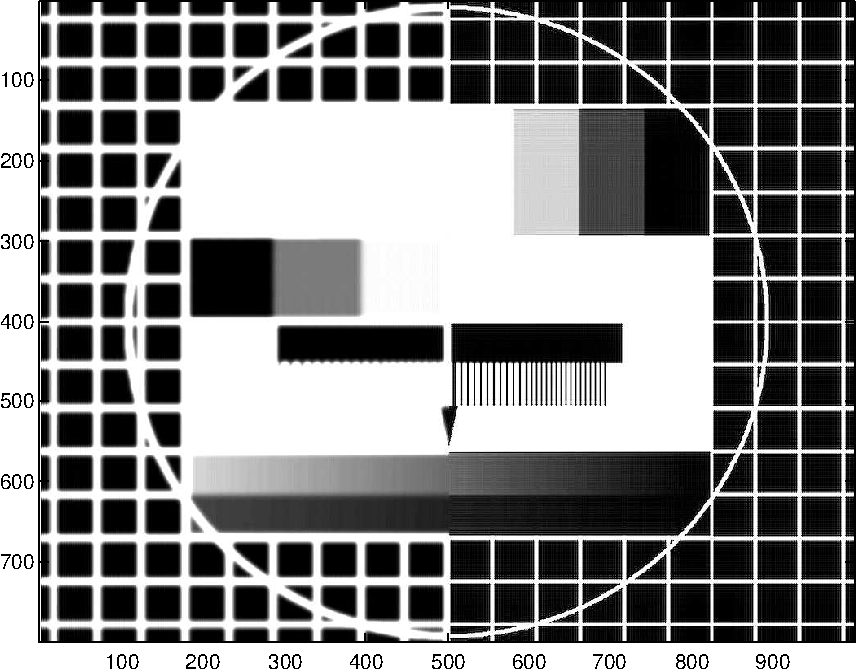
\includegraphics[width=0.7\textwidth,keepaspectratio]{../tmp/eins_c_0_5-crop.pdf}
  \caption{Bild mit Rand bei $ρ^2 = 0.5$}
  \label{fig:pic_trafo_0_5}
\end{figure}

Im Vergleich zu \fref{1a} kann man erkennen, dass, abgesehen davon, dass kein
Rahmen zum Bild hinzugefügt wurde, das Bild selbst verändert wurde. 

\section*{Aufgabe 5.1d)}
Hier wurde der Schnitt auf den Betrag von $k$ angewandt und nicht wie bisher
auf die einzelnen Komponenten. Der aufrufende Quelltext ist in \lref{k_kreis} und 
die aufgerufene Funktion \texttt{cut\_round} dargestellt.

\lstinputlisting[firstline=32,firstnumber=32,label=lst:k_kreis,caption={blatt5.m}]{../code/blatt5.m}
\lstinputlisting[label=lst:cut_round,caption={cut\_round.m}]{../code/cut_round.m}

Die hierbei resultierenden Graphiken sind in \fref{kreis_0_1} (für $k = 0.1$) und
\fref{kreis_0_5} (für $k=0.5$) dargestellt.

\begin{figure}[htb]
\centering
  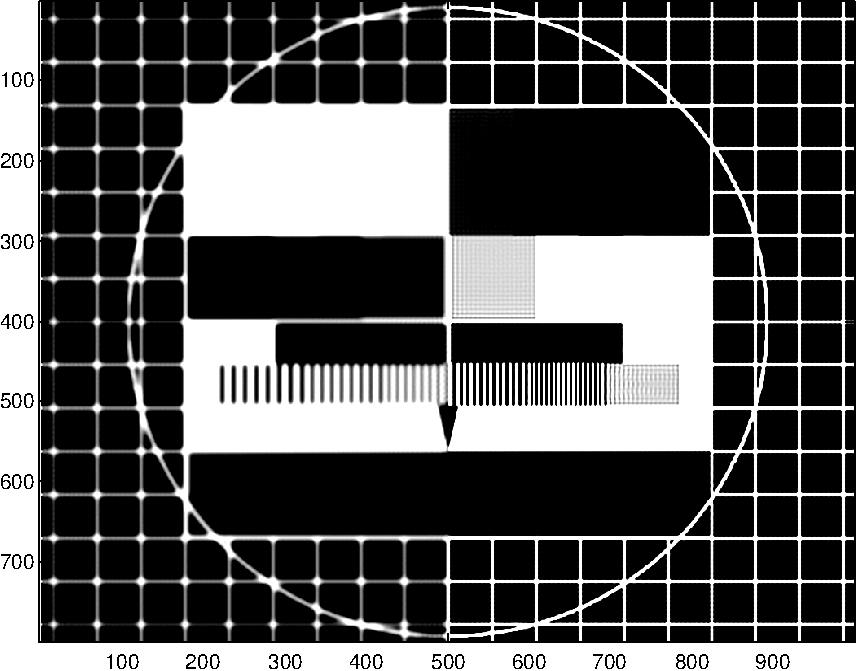
\includegraphics[width=0.7\textwidth,keepaspectratio]{../tmp/eins_d_0_1-crop.pdf}
  \caption{Bild mit Rand bei $ρ^2 = 0.1$}
  \label{fig:kreis_0_1}
\end{figure}

\begin{figure}[htb]
\centering
  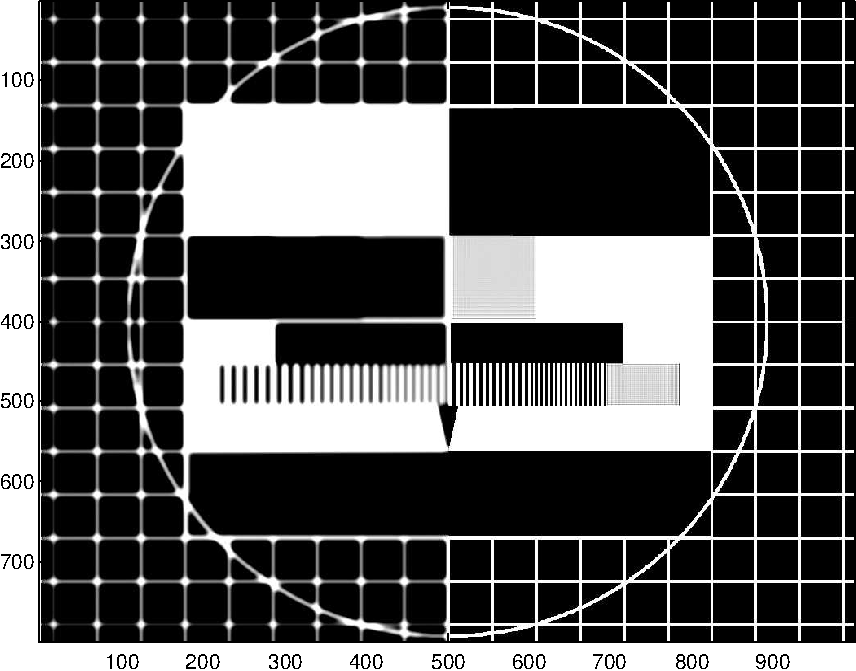
\includegraphics[width=0.7\textwidth,keepaspectratio]{../tmp/eins_d_0_5-crop.pdf}
  \caption{Bild mit Rand bei $ρ^2 = 0.5$}
  \label{fig:kreis_0_5}
\end{figure}

Die unterschiedlichen Werte für ϱ äußern sich hier in ein wenig anderen Artefakten. 
Die beiden hellgrauen Blöcke in der rechten Mitte der Bilder sind für $ϱ²=0.5$
annähernd homogen ausgefüllt, während für $ϱ²=0.1$ eine deutliche Strukturierung
zu erkennen ist. Im ursprünglichen Bild waren diese Bereiche homogen (oberer Block)
oder vertikal gestreift (unterer Block). Eine geringere Beschneidung im $k$-Raum
führt also zu einer tendenziell größeren Erhaltung der Informationen, was auch zu
erwarten war.

\section*{Aufgabe 5.1e)}